\section{Das Reflektionsprinzip}

Wir betrachten f�r $a > 0$ die erste Passierzeit $\tau_a := \inf\{t \geq 0 : W_t = a\}$ und wollen untersuchen, wie die Verteilung oder Verteilungsfunktion von $\tau_a$ aussieht. Wegen $P(W_t = a) = 0$ gilt zun�chst $P(\tau_a \leq t) = P(\tau_a \leq t, W_t \geq a) + P(\tau_a \leq t, W_t \leq a)$. Ferner gilt $P(\tau_a \leq t, W_t \geq a) = P(W_t \geq a)$, da mit $W_0 = 0$ $P$-fast sicher und der Stetigkeit der Pfade folgt, dass $\{W_t \geq a\} \subset \{\tau_a \leq t\}$ gilt. F�r den zweiten Summanden wollen wir nun eine heuristische Betrachtung durchf�hren:

\begin{figure}[!htbp]
\centering
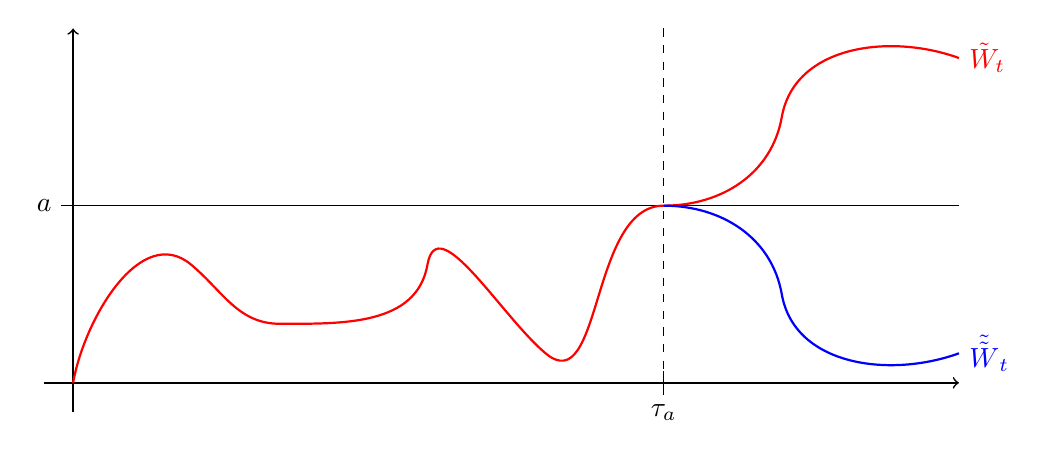
\begin{tikzpicture}[scale=0.75]
\draw[semithick, ->] (-0.5,0) -- (15,0);
\draw[semithick, ->] (0,-0.5) -- (0,6);

\draw (-0.2, 3) node[left] {$a$} -- (15, 3);
\draw (10, 0.2) -- (10, -0.2) node [below] {$\tau_a$};
\draw[dashed] (10, 6) -- (10, 0.2);

\draw[thick, red] (0, 0)   to[out=80, in=140]
									(2, 2)   to[out=-40, in=180]
									(3.5, 1) to[out=0, in=-100]
									(6, 2)   to[out=80, in=140]
									(8, 0.5) to[out=-40, in=180]
									(10, 3);
									
\draw[thick, red] (10, 3)   to[out=0, in=-100]
									(12, 4.5) to[out=80, in=160]
									(15, 5.5) node[right] {$\tilde{W}_t$};
\draw[thick, blue](10, 3)   to[out=0, in=100]
									(12, 1.5) to[out=-80, in=-160]
									(15, 0.5) node[right] {$\tilde{\tilde{W}}_t$};
\end{tikzpicture}
\caption[Neugestarteter Prozess f�r das Reflektionsprinzip]{Der Prozess wird in $\tau_a$ neugestartet und ist dann um $a$ gewisserma�en symmetrisch.}\label{fig:reflektionsprinzip}
\end{figure}

Wir starten den Wiener-Prozess in $\tau_a$ neu, nach Satz \ref{Nummer5.3.6} ist die Zukunft dann von der Vergangenheit bis $\tau_a$ unabh�ngig. Der neugestartete Wiener-Prozess ist zudem gewisserma�en um die $a$ symmetrisch, d.\,h. $W$ und $-W$ sind Wiener-Prozesse. Damit ist
\begin{align*}
P(\tau_a \leq t, W_t \leq a) &= P(\tau_a \leq t, \tilde{W}_t \leq a) \stackrel{\text{!}}{=} P(\tau_a \leq t, \tilde{\tilde{W}}_t \geq a) = P(\tilde{\tilde{W}}_t \geq a) = P(W_t \geq a)\text{.}
\end{align*}
Insgesamt gilt also $P(\tau_a \leq t) = 2P(W_t \geq a)$. Die markierte Gleichheit bei $\stackrel{\text{!}}{=}$ ist so jedoch nicht begr�ndbar, da Symmetrie eigentlich eine andere Eigenschaft ist. Um dies zu reparieren, ben�tigen wir den folgenden Satz.

\begin{satz}\label{Nummer5.4.1}
Mit den obigen Bezeichnungen ist $(\tilde{W}_t)_{t \geq 0}$ definiert durch
\begin{align*}
\tilde{W}_t &:= \begin{cases} W_t & \text{falls } t \leq \tau_a\\ 2a - W_t & \text{sonst}\end{cases}
\end{align*}
ebenfalls ein Wiener-Prozess.
\end{satz}

\begin{beweis}
Wegen Satz \ref{Nummer5.3.6} definiert $X_t := W_{t + \tau_a} - W_{\tau_a}$ einen von $\sF_{\tau_a}$ unabh�ngigen Wiener-Prozess. Damit haben $X := (X_t)$, $(-X_t)$ und $W := (W_t)$ die selben Verteilungen und es gilt $X \stackrel{[d]}{=} -X \stackrel{[d]}{=} W$. Ferner ist $X$ von der $\sF_{\tau_a}$-messbaren Zufallsvariablen $\tau_a$ unabh�ngig. Wegen $\tau_a \wedge s \leq \tau_a$ f�r $s \geq 0$ gilt $\sF_{\tau_a \wedge s} \subset \sF_{\tau_a}$ und damit ist $Y := (W_{\tau_a \wedge s})_{s \geq 0}$ nach Satz \ref{Nummer5.3.5} und Lemma \ref{Nummer5.3.4} ein $(\sF_{\tau_a \wedge s})_{s \geq 0}$-adaptierter Prozess. Wegen $\sF_{\tau_a \wedge s} \subset \sF_{\tau_a}$ ist dann $X$ von $Y$ unabh�ngig und da $(Y, \tau_a)$ von $X$ bzw. $-X$ unabh�ngig ist, erhalten wir
\begin{align*}
(Y, \tau_a, X) &\stackrel{[d]}{=} (Y, \tau_a, -X)\text{.} \tag{*}
\end{align*} 
Wir betrachten nun $C_0 := \{g \in C([0, \infty))\text{, } g(0) = 0\}$ und $\psi\colon C([0, \infty)) \times [0, \infty) \times C_0 \to C([0, \infty))$ definiert durch
\begin{align*}
\psi(f, t_0, g) &:= \begin{cases} f(t) & \text{falls } t \leq t_0\\ f(t_0) + g(t-t_0) & \text{falls } t \geq t_0\end{cases}
\end{align*}
f�r alle $t \geq 0$. Mit (*) erhalten wir dann $\psi(Y, \tau_a, X) \stackrel{[d]}{=} \psi(Y, \tau_a, -X)$. Ferner ist
\begin{align*}
\psi(Y, \tau_a, X) &= \begin{cases}W_t & \text{falls } t \leq \tau_a\\ W_{\tau_a} + X_{t-\tau_a} & \text{falls } t \geq \tau_a\end{cases}\\
\quad &= (W_t)_{t \geq 0}
\shortintertext{und analog}
\psi(Y, \tau_a, -X) &= \begin{cases}W_t & \text{falls } t \leq \tau_a\\ W_{\tau_a} - X_{t-\tau_a} & \text{falls } t \geq \tau_a\end{cases}\\
\quad &= W_{\tau_a} - W_{\tau_a + t - \tau_a} + W_{\tau_a} = 2a - W_t\\
\quad &= (\tilde{W}_t)_{t \geq 0}\text{.}
\end{align*}
Damit besitzen $(W_t)$ und $(\tilde{W}_t)$ die gleichen Verteilungen und daher ist $(\tilde{W}_t)$ ein zentrierter Gau�-Prozess mit der Kovarianzfunktion $\Gamma(s,t) = \min\{s, t\}$, der nach Konstruktion stetige Pfade besitzt, also ist er ein Wiener-Prozess.
\end{beweis}

\begin{satz}[Reflektionsprinzip]\label{Nummer5.4.2}
Sei $(W_t)$ ein Wiener-Prozess und $\tau_a$ die erste Passierzeit f�r ein $a > 0$. Dann gilt
\begin{align*}
P\left(\max_{s \in [0, t]} W_s \geq a\right) &= P(\tau_a \leq t) = P(\vert W_t \vert \geq a) = 2P(W_t \geq a)\\
\quad &= 1 - \sN(0,t)[-a,a]\text{.}
\end{align*}
\end{satz}

Man kann ferner zeigen, dass $P$-fast sicher $\tau_a < \infty$ gilt, was unmittelbar aus den Aussagen des Satzes folgt. Die Dichte von $\tau_a$ l�sst sich auch bestimmen, hierzu verweisen wir auf \cite[Satz 13.9]{MEINTRUP}. Schlie�lich l�sst sich auch $\E \tau_a = \infty$ zeigen.

\begin{information}
Satz \ref{Nummer5.4.1} wird h�ufig ebenfalls oder alternativ Reflektionsprinzip genannt.
\end{information}

\begin{beweis}
Man kann leicht zeigen, dass $\{\tau_a \leq t\} = \left\{\max_{s \in [0,t]} W_s \geq a\right\}$ gilt. Damit reicht es, zu zeigen, dass
\begin{align*}
P\left(\max_{s \in [0,t]} W_s \geq a\right) &= 2P(W_t \geq a)
\end{align*}
gilt. Dazu sei $(\tilde{W}_t)$ der Wiener-Prozess aus Satz \ref{Nummer5.4.1}. Dann gilt $\{W_t \geq a\} \subset \{\tilde{W}_t \leq a\}$ und analog f�r $>$ und $<$, denn f�r $W_t \geq a$ gilt $\tau_a \leq t$ und damit $\tilde{W}_t = 2a - W_t \leq 2a-a = a$. Ferner erhalten wir eine disjunkte Vereinigung
\begin{align*}
\left\{\max_{s \in [0,t]} W_s \geq a\right\} &= \{W_t \geq a\} \sqcup \{\tilde{W}_t > a\}\text{,}
\end{align*}
dazu sei f�r "`$\subset$"' zun�chst $s \in [0,t]$ mit $W_s \geq a$, dann gilt entweder $W_t \geq a$ und wir sind fertig oder es gilt $W_t < a$. In diesem Fall folgt mit dem Zwischenwertsatz $\tau_a \leq s \leq t$ und damit $\tilde{W}_t = 2a - W_t > 2a-a = a$. F�r "`$\supset$"' beobachten wir zun�chst, dass $\{W_t \geq a\} \subset \left\{\max_{s \in [0,t]} W_s \geq a\right\}$ offensichtlich ist. Sei nun $\tilde{W}_t > a$, dann folgt mit unseren Vor�berlegungen $W_t < a$. Damit gilt $\tilde{W}_t \neq W_t$ und aus der Definition von $\tilde{W}_t$ folgt daher $t > \tau_a$. Dann existiert ein $s \in [0,t]$ mit $W_s = a$ und daher $\max_{s \in [0,t]} W_s \geq a$. 

Damit gilt nun
\begin{align*}
P\left(\max_{s \in [0,t]} W_s \geq a\right) &= P(W_t \geq a) + P(\tilde{W}_t > a) = P(W_t \geq a) + P(\tilde{W}_t \geq a)\\
\quad &= 2P(W_t \geq a)\text{.} \qedhere
\end{align*}
\end{beweis}